% main.text
\documentclass[12pt, a4paper]{article}
\usepackage{graphicx}
\graphicspath{ {images/} }
\input \jobname
\title{CE 388}
\date{March 2020}

\begin{document}
\maketitle

\begin{figure}[h]
    \centering
    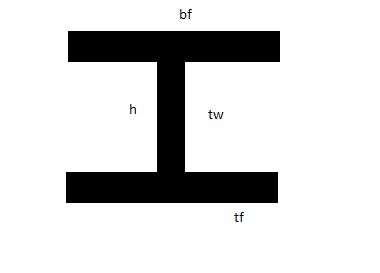
\includegraphics[width=0.75\textwidth]{theimage}
    \caption{a nice plot}
    \label{fig:mesh1}
\end{figure}

Name: \varZero\

Surname: \varOne\

ID Number: \varTwo\

Proporties of the steel section: tf = \varThree\ , bf = \varFour\ , tw = \varFive\ and h = \varSix\ . Please calculate moment of inertia of the given section.


\end{document}

%for %i in (*) do pdflatex -jobname=%i main.tex